%\usepackage{amsmath}
%\usepackage{hyperref}
%\usepackage{amsthm}
%\usepackage{graphicx}
\documentclass[journal, a4paper]{IEEEtran}
\usepackage[italian]{babel}
\usepackage{booktabs}
\usepackage{siunitx}%Questo serve a caricare il pacchetto delle unità di misura del sistema internazionale%
\usepackage[utf8]{inputenc}
\usepackage{graphicx} 
\usepackage{url}
\usepackage{amsmath}
\usepackage{amssymb}


\usepackage{keyval}
\usepackage{xcolor}
\usepackage{caption}
\usepackage{subfig}
\usepackage{tikz}
\usepackage{circuitikz}
\usepackage{authblk}
%\usepackage{hyperref}

\begin{document}


% Define document title and author
	\title{Tecnologie Digitali - Logbook Week 9}
	\author[1]{Salvatore Bottaro}
		\author[2]{Lorenzo M. Perrone}
		\affil[1]{\texttt{salvo.bottaro@hotmail.it}}
		\affil[2]{\texttt{lorenzo.perrone.lmp@gmail.com}}
	\markboth{Tecnologie Digitali - Di Lieto}{}
	\maketitle
	
\begin{abstract}
	Logbook di laboratorio di Tecnologie Digitali, a.a. 2015/2016. Week 9.
\end{abstract}

\section{Funzioni logiche di base}

L'elettronica digitale è caratterizzata dal fatto he essa impiega segnali che assumono due valori ben distinti, identificati con 0 e 1 o con \emph{falso} e \emph{vero}. Le uniche funzioni logiche ad un ingresso sono la negazione \textbf{NOT} e l'identità \textbf{I}. Quelle a due ingressi sono \textbf{AND}, \textbf{NAND}, \textbf{OR}, \textbf{NOR}, \textbf{XOR}, \textbf{XNOR} i cui simboli sono rappresentati in figura \ref{fig:logic}. 

\begin{figure}[htp]
\centering
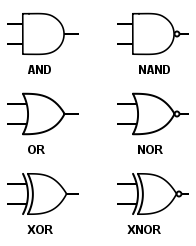
\includegraphics[scale=.55]{logic}
\caption{Simboli delle funzioni logiche a due ingressi}
\label{fig:logic}
\end{figure}

Ciascuna funzione logica è definita da una tavola della verità. Per costruire quelle delle funzioni a due ingressi basta limitarsi alle funzioni \textbf{AND}, \textbf{OR}, \textbf{XOR} (tabella~\ref{tab:logic}) poichè le altre si ottengono applicando l'operatore \textbf{NOT} a quelle precedenti.

\begin{table}[htp]
\centering
\caption{Tavole delle verità delle funzioni logiche principali.}
\label{tab:logic}
\begin{tabular}{|c|c|c|c|c|}
\hline 
A & B & AND(A,B) & OR(A,B) & XOR(A,B) \\ 
\hline 
T & T & T & T & F \\ 
\hline 
T & F & F & T & T \\ 
\hline 
F & T & F & T & T \\ 
\hline 
F & F & F & F & F \\ 
\hline 
\end{tabular} 
\end{table}

\section{Segnali logici della scheda di acquisizione}

La scheda National presenta 8 porte logiche che fungono sia da ingressi che da uscite, indicati con DIOx. In particolare i canali 0-3 corrispondono rispettivamente alle CB52, CB17, CB49, CB47. Abbiamo misurato con il tester analogico i livelli di tensione corrispondenti ai 2 possibili stati logici delle porte prima menzionate, i risultati delle misure son raccolti in tabella \ref{tab:volt}.

\begin{table}[htp]
\centering
\caption{Tensioni di uscita delle porte logiche impiegate.}
\label{tab:volt}
\begin{tabular}{|c|c|c|}
\hline 
Porta & True (V) & False (mV)\\ 
\hline 
CB52 & 5.05 & 1.7 \\ 
\hline 
CB17 & 5.05 & 1.6 \\ 
\hline 
CB49 & 5.05 & 1.5 \\ 
\hline 
CB47 & 5.05 & 1.7 \\ 
\hline 
\end{tabular} 
\end{table}

Per verificare il corretto dunzionamento delle porte digitali abbiamo impiegato un tester digitale ostituito da un connettore DIL che collega un \emph{flat-cable} da montare sulla breadboard ad una serie di LED. Questi sono connessi ai pin 2-5 e 10-13, il pin 14 corrisponde alla terra. Abbiamo dunque connesso le porte digitali DIO0-3 ai pin 2-5 del tester digitale e abbiamo verificato che i LED si accendevano e spegnevano corrispondentemente allo stato logico delle porte digitali impostato tramite il VI \texttt{Digital$\_$out4}.

\section{Circuiti base}

In figura \ref{fig:14011} è riportata la zoccolatura dell'integrato 14011 contenente 4 porte \textbf{NAND} a due ingressi della famiglia CMOS.

\begin{figure}[htp]
\centering
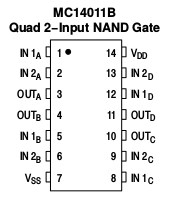
\includegraphics[scale=0.8]{pinscheme}
\caption{Zoccolatura del 14011.}
\label{fig:14011}
\end{figure}

In tabella \ref{tab:data} sono riportate le altre caratteristiche rilevanti del 14011 presenti sul datasheet.

\begin{table}
\centering
\caption{Caratteristiche del 14011}
\label{tab:data}
\begin{tabular}{|c|c|c|}
  \hline
  Grandezza & $V_{DD}$ (V)& Valore \\
  \hline
           &  5  &  0.05 V \\ \cline{2-3}
  $V_{OL}$ & 10  &  0.05 V \\ \cline{2-3}
           & 15  &  0.05 V \\ 
  \hline 
           &  5  &  4.95 V \\ \cline{2-3}
  $V_{OH}$ & 10  &  9.95 V \\ \cline{2-3}
           & 15  & 14.95 V \\ 
  \hline \hline
           &  5  &  1.5 V \\ \cline{2-3}
  $V_{IL}$ & 10  &  3.0 V \\ \cline{2-3}
           & 15  &  4.0 V \\ 
  \hline 
           &  5  &  3.5 V \\ \cline{2-3}
  $V_{IH}$ & 10  &  7.0 V \\ \cline{2-3}
           & 15  &   11 V \\ 
  \hline \hline
           &  5  &  -0.51 mA \\ \cline{2-3}
  $I_{OH}$ & 10  &  -1.3  mA \\ \cline{2-3}
           & 15  &  -3.4  mA \\ 
  \hline 
           &  5  &  0.51 mA \\ \cline{2-3}
  $I_{OL}$ & 10  &  1.3  mA \\ \cline{2-3}
           & 15  &  3.4  mA \\
  \hline \hline
  $I_{in}$ & 15  &  $\pm$ 0.1 $\mu$A\\
  \hline \hline
  $P_D$    & -   &  500 mW\\
  \hline \hline
            &  5  &  200  ns \\ \cline{2-3}
  $t_{TLH}$ & 10  &  100  ns \\ \cline{2-3}
            & 15  &   80  ns \\
  \hline 
            &  5  &  200  ns \\ \cline{2-3}
  $t_{THL}$ & 10  &  100  ns \\ \cline{2-3}
            & 15  &   80  ns \\
  \hline
  $t_{PLH}$, &  5  &  125  ns \\ \cline{2-3}
  $t_{PHL}$  & 10  &   50  ns \\ \cline{2-3}
             & 15  &   40  ns \\
  \hline
\end{tabular}
\end{table}

In figura \ref{fig:response} sono definiti i vari tempi di risposta del dispositivo.

\begin{figure}[htp]
\centering
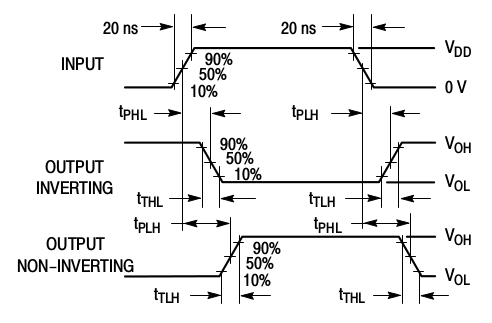
\includegraphics[scale=.5]{response}
\caption{Definizione dei vari tempi di risposta.}
\label{fig:response}
\end{figure}

Si è verificata la funzionalità del 14011 collegando l'uscita di ciascuna delle 4 porte ad un LED e ricostruendone tramite il \texttt{Digital$\_$out4} le tavole di verità, ritrovando in tutti e 4 i casi la tavola di verità della funzione \textbf{NAND}.\\

Abbiamo scollegato poi una delle due porte logiche dal dispositivo per osservare cosa succede quando un ingresso non è collegato ad un segnale valido, mantenendo quello collegato sullo stato \textit{vero}. Con il tester logico abbiamo osservato che in alcuni casi cambiano lo stato della porta collegata da falso a vero il LED rimaneva acceso per qualche secondo per poi spegnersi. Inizialmente avevamo attribuito tale comportamento a fenomeni capacitivi, tuttavia altre prove hanno escluso questa ipotesi, fra cui quella in cui il LED dopo ssersi spento si è riacceso. Collegando il tester analogico e cambiando lo stato della porta collegata, abbiamo osservato che ogni volta che lo stato in input era vero, quello in uscita era falso, ovvero come se il 14011 leggesse l'ingresso non valido come vero. Infine tramite il VI \texttt{Acquis$\_$Base} abbiamo misurato l'uscita della porta al variare del tempo. Abbiamo dapprima campionato l'uscita senza modificare l'ingresso scollegato. I dati sono in figura \ref{fig:es81}, come si vede il segnale rilevato è costantemente falso al variare del tempo, quindi l'ingresso scollegato è stato letto come vero.

\begin{figure}[htp]
\centering
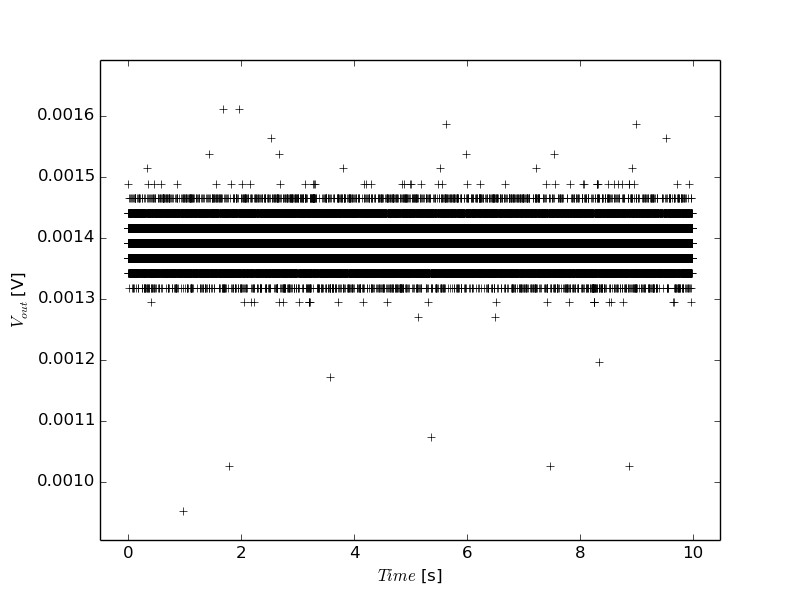
\includegraphics[scale=.4]{es8_vero17}
\caption{Segnale all'uscita della porta cn uno dei due ingressi scollegato.}
\label{fig:es81}
\end{figure}

Abbiamo fatto poi altre prove acquisendo il segnale in uscita cambiando lo stato dell'ingresso scollegato, ovvero collegandolo e scollegandolo dalla terra più volte nel corso dell'acquisizione. La prima prova è stata fatta mantenendo scollegato l'ingresso, per poi collegarlo a terra e successivamente riscollegarlo. Il segnale in uscita è in figura \ref{fig:es82}: il salto corrisponde all'inserimento della terra, ma non c'è traccia del successivo scollegamento.

\begin{figure}[htp]
\centering
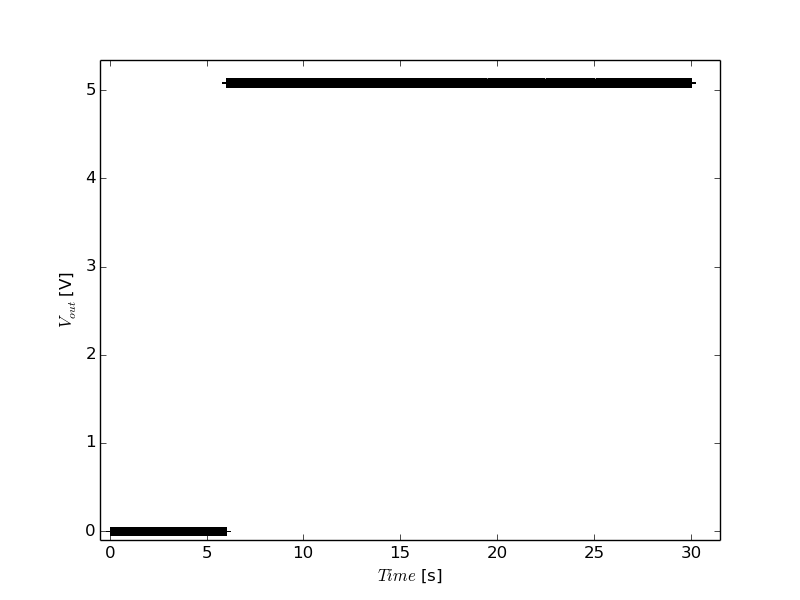
\includegraphics[scale=.4]{es8_falso-veroboh2}
\caption{Segnale all'uscita della porta cambiando lo stato di un ingresso inizialmente scollegato.}
\label{fig:es82}
\end{figure}

Una seconda prova è stata fatta tenendo inizialmente la terra collegata e scollegandola e ricollegandola ogni 5 secondi. In figura \ref{fig:es83} sono mostrati i dati: a parte una serie di dati allineati verticalmente in corrispondenza del primo scollegamento, non c'è traccia dei successivi. Probabilmente se avessimo tenuto scollegata la terra più a lungo il segnale sarebbe cambiato, in quanto la persistenza di un certo segnale è dovuto ad un accumulo di carica che fa sì che il segnale letto in ingresso sia vero, per cui quando si collega il segnale a terra ovviamente tale accumulo si scarica, per poi impiegare un certo tempo per ricaricarsi.

\begin{figure}[htp]
\centering
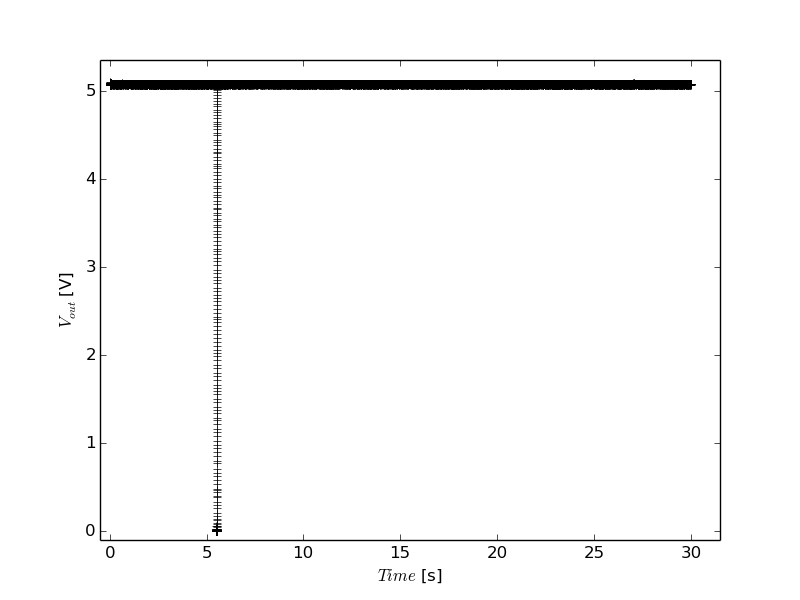
\includegraphics[scale=.4]{es8_falso-veroboh}
\caption{Segnale all'uscita della porta cambiando lo stato di un ingresso inizialmente a terra.}
\label{fig:es83}
\end{figure}

\section{Realizzazione di circuiti logici combinazionali}

Cortocircuitando gli ingressi di una porta \textbf{NAND}, si realizza il circuito in figura \ref{fig:not}. L'equazione logica risulta essere:
\begin{equation}
\overline{A \cdot A} = Q
\end{equation}
ma poiché $A \cdot A = A$, si ha:
\begin{equation}
\overline{A \cdot A} =\bar{A}
\end{equation}
ovvero il circuito dovrebbe funzionare come un circuito \textbf{NOT}, difatti tramite tester logico si è verificato che l'uscita restituisce l'opposto dello stato in ingresso, ovvero il circuito così realizzato è proprio un circuito \textbf{NOT}.  

\begin{figure}[htp]
\centering
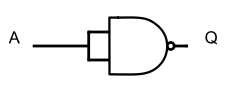
\includegraphics[scale=.6]{not}
\caption{Schema logico del circuito NOT.}
\label{fig:not}
\end{figure}

Dal momento che la funzione \textbf{AND} si ottiene negando \textbf{NAND}, si ottiene immediatamente da quanto visto in precedenza lo schema per un circuito \textbf{AND} in figura \ref{fig:and}. Si è verificato sperimentalmente che il circuito così realizzato si comporta come un circuito \textbf{AND}.

\begin{figure}[htp]
\centering
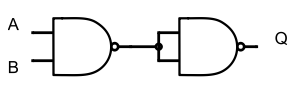
\includegraphics[scale=.6]{and}
\caption{Schema logico del circuito AND.}
\label{fig:and}
\end{figure}

Dato il circuito in figura \ref{fig:or}, lo abbiamo realizzato sulla breadboard e costruito la tavola della varità. 

\begin{figure}[htp]
\centering
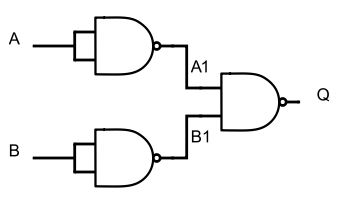
\includegraphics[scale=.6]{or}
\caption{Schema logico del circuito OR.}
\label{fig:or}
\end{figure}

Si è ottenuta quella della funzione \textbf{OR}, come si poteva prevedere applicando le leggi di De Morgan. Infatti l'equazione del circuito è:

\begin{equation}
\overline{\bar{A} \cdot \bar{B}} = \overline{\overline{A + B}} = A + B.
\end{equation}

Dal circuito \textbf{OR} si passa immediatamente al circuito \textbf{NOR} aggiungendo un circuito \textbf{NOT} alla fine, come si vede in figura \ref{fig:nor}.

\begin{figure}[htp]
\centering
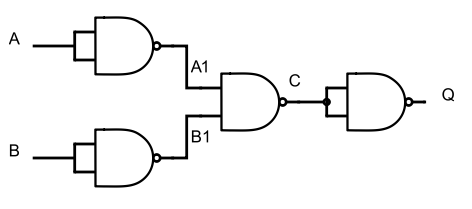
\includegraphics[scale=.5]{nor}
\caption{Schema logico del circuito NOR.}
\label{fig:nor}
\end{figure}

Abbiamo realizzato sulla breadboard il circuito in figura \ref{fig:xor} e costruito la tavola di verità. Ciò che si è ottenuto è stata quella della funzione \textbf{XOR}.

\begin{figure}[htp]
\centering
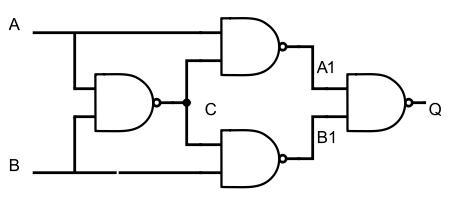
\includegraphics[scale=.5]{xor}
\caption{Schema logico del circuito XOR.}
\label{fig:xor}
\end{figure}

Infatti applicando le leggi di De Morgan:
\begin{equation}
\begin{split}
Q & = \overline{(\overline{B \cdot \overline{A \cdot B}})\cdot (\overline{A \cdot \overline{A \cdot B}})} \\
  & = B \cdot \overline{A \cdot B} + A \cdot \overline{A \cdot B} \\
  & =(\bar{A} + \bar{B})\cdot B + (\bar{A} + \bar{B})\cdot A \\
  & = \bar{A}\cdot B + \bar{B} \cdot A \\
\end{split}
\end{equation}

che è la definizione della funzione \textbf{XOR}.

\section{Logica NOR}



\end{document}